\documentclass{article}

\usepackage[preprint]{neurips_2026}  % preprint mode: non-anonymous, for arXiv-style posting, not a conference double-blind submission

\usepackage[utf8]{inputenc}
\usepackage[T1]{fontenc}
\usepackage{hyperref}
\usepackage{url}
\usepackage{booktabs}
\usepackage{amsfonts}
\usepackage{amsmath}
\usepackage{amssymb}
\usepackage{nicefrac}
\usepackage{microtype}
\usepackage{xcolor}
\usepackage{graphicx}

\title{On the Sufficiency of Observable State for Chain-of-Thought Early Stopping}

\author{%
  Sneh Kansagara \\
  ABV-Indian Institute of Information Technology and Management, Gwalior \\
  \texttt{snehkansagara@gmail.com} \\
}

\begin{document}

\maketitle

\begin{abstract}
Training-free chain-of-thought early-stopping methods all decide whether to halt generation based on a reasoning trajectory's \emph{current} observable state, meaning its present answer, token confidence, and predictive entropy. Every such method implicitly assumes this state is a sufficient statistic for the trajectory's eventual answer. This assumption is load-bearing for the entire family of such methods, yet to our knowledge it has never been tested directly, only used. We test it. Using a pre-registered, power-analyzed matched-pair natural-branching design, we identify pairs of reasoning prefixes from the same problem, but different trajectories, that already agree on observable state, and let each side continue naturally many times to see whether their future-answer distributions diverge beyond what sampling noise predicts. We call this phenomenon \emph{path dependence}. We report our findings at two tiers of confidence, matched to where our data actually supports each claim. \textbf{At the semantic level (answer-only matching, which we call L1), our evidence is robust.} Across a pre-registered, well-powered 21-pair primary sample ($\sim$89\% power for our target effect size, on DeepSeek-R1-Distill-Qwen-7B and MATH-500) and an independent 45-pair scale-up, 56 of 66 matched pairs converge to \emph{exactly} identical future-answer distributions regardless of history, and the combined test across all 66 pairs is far from significant. Three pairs from the primary sample reach nominal significance. Converging evidence, including a Bonferroni correction, non-replication on independent redraws of the same two problems, and the scale-up's null result, indicates these three pairs are consistent with sparse-sample noise rather than a stable effect. \textbf{At the richer, epistemic-state level (confidence and entropy beyond the answer alone), our evidence is directional, not confirmatory.} A continuous regression of divergence against state-space distance, the statistically stronger test for this question, is also null ($p=0.47$), but is scoped to the smaller, reduced-branch-budget portion of our data ($n=45$ pairs at $N=10$ branches per pair, versus the primary sample's $N=40$) and should be read as consistent with, not independent confirmation of, the semantic-level result. We also test whether a stopping rule built directly on this paper's own findings, which we call Sufficiency-Gated Early Stopping, improves on the simplest possible baseline, a fixed-fraction cutoff. It does not. Additional state-matching sophistication bought no accuracy or efficiency gain over the naive rule. Taken together, these results are evidence \emph{for} the assumption the early-stopping literature has been making implicitly. Within the scope we test, current observable state behaves as a sufficient statistic for a reasoning trajectory's eventual answer, most strongly at the semantic level and suggestively at the richer epistemic-state level, and the field's methods do not appear to be leaving exploitable historical information on the table. We report this scoped to one model and one domain, and are explicit about what a null result of this kind can and cannot establish.
\end{abstract}

\section{Introduction}
\label{sec:intro}

Chain-of-thought reasoning is expensive, and a growing body of work tries to cut that cost by stopping generation as soon as a model has effectively decided its answer, without any additional training. Our own earlier pilot on this model illustrates why the idea is attractive: MATH-500 accuracy is \emph{non-monotonic} in trace length. Truncating generation to 75\% of its natural length measured 7.5 points \emph{higher} accuracy than letting the model run to completion. Reasoning models sometimes talk themselves out of answers they already had. If a stopping rule can reliably tell when that point has been reached, it saves both compute and accuracy.

Every training-free method for making that call, whether it compares current answer stability, token confidence, predictive entropy, or some combination of the three against a threshold, makes the same implicit assumption. This \textbf{current observable state} is treated as what the decision should be based on, because it already captures everything relevant about where the trajectory is headed. Two trajectories that currently look identical to the stopping rule are treated as interchangeable from that point forward. This assumption is never stated as a hypothesis, let alone tested. It is simply the feature space these methods are built on.

We ask directly: \textbf{is a reasoning trajectory's current observable state, meaning its answer, confidence, and entropy, actually a sufficient statistic for its eventual answer, or does the \emph{history} that produced that state carry additional predictive information the stopping rule is throwing away?} We call the latter possibility \emph{path dependence}. Two prefixes agree on observable state now, but diverge in their future-answer distribution beyond what sampling noise alone would predict, because of where they came from rather than where they currently are. Put plainly, early-stopping methods treat reasoning trajectories as effectively Markovian with respect to observable state. This paper is a direct empirical test of that assumption, not merely a use of it.

To test this, we identify pairs of prefixes, from the same problem but different reasoning trajectories, matched on observable state at matched depth, and let each side continue naturally many times, measuring whether their resulting answer distributions differ more than a matched permutation null predicts. We run this at three matching strictnesses, from answer-only (the loosest, closest to what a pure answer-stability detector sees) to answer-plus-confidence-plus-entropy (the strictest). A gap found only at the loosest level and closed by richer state would itself be an informative, actionable result, not a failure to detect path dependence, but a demonstration of exactly which signal a stopping rule needs to track to avoid it.

\textbf{Our central finding is a well-powered, convergent null across every independent test we ran.} Across a pre-registered 21-pair primary sample ($\sim$89\% power for the effect size we targeted) and a 45-pair scale-up collected afterward at a reduced per-pair branch budget, we find no aggregate evidence of path dependence. 56 of 66 matched pairs go on to produce \emph{exactly} identical answer distributions regardless of history, and the combined test across all pairs is far from significant. A small number of individual pairs reach nominal significance in the primary sample, but this does not survive scrutiny. It fails Bonferroni correction in the pooled 66-pair set, both flagged problems fail to replicate on an independently sampled second pair, and, most directly, a continuous regression of divergence against state-space distance, the statistically stronger test our own analysis library was built to run, is itself null ($p=0.47$) once we finally collected the state data needed to run it. We read this convergence, not any single test alone, as the paper's evidence. Current observable state behaves as a sufficient statistic within the scope we test, and the assumption early-stopping methods have been making implicitly survives a direct, adversarially designed attempt to break it.

\textbf{Contributions:}
\begin{enumerate}
  \item The first direct empirical test, to our knowledge, of whether current observable state is a sufficient statistic for a reasoning trajectory's future answer, the Markovian assumption underlying the entire family of training-free early-stopping methods, via a pre-registered, power-analyzed, matched-pair natural-branching design, corroborated by an independent scale-up and, for the first time, the continuous state-distance regression this design was always meant to support.
  \item Evidence, not proof: a well-powered null result that is consistent with current state being sufficient, reported with the scope (one model, one domain, one matching regime) and statistical limits that determine what a null result of this kind can and cannot establish.
  \item A direct test of the practical implication: a stopping rule built on this paper's own findings does not outperform the simplest possible fixed-fraction baseline on either accuracy or token savings, suggesting that state-matching sophistication beyond simple answer and confidence extraction is not obviously buying anything in this regime.
  \item A transparent account of every place our own execution fell short of its pre-registered design (matching-level coverage in the primary sample, achieved sample size, reduced branch budget in the scale-up), so the result is legible about its own limits rather than presented as more definitive than the data supports.
\end{enumerate}

\section{Related Work}
\label{sec:relatedwork}

\paragraph{Training-free early-stopping for chain-of-thought reasoning.} A growing line of work detects when a reasoning trajectory has effectively decided its answer and halts generation early, without any additional training. REFRAIN \citep{refrain2026} segments traces on the same blank-line convention we use and benchmarks a broad family of such signals (No-thinking, DEER, HALT-CoT, CoT-Valve, Deepconf) against each other. Statistical Early Stopping for Reasoning Models \citep{statisticalearlystopping2026} frames the problem statistically and reports recovering roughly 82 to 85\% of an oracle stopping policy's power. ThinkBrake \citep{thinkbrake2026} constructs its oracle via forced termination and shows an 8\% accuracy gain and a 72\% token reduction against it. \textbf{All of these methods, and the broader family they represent, share the same implicit assumption this paper tests directly}, that the trajectory's current observable state is what the stopping decision should, and safely can, be based on. None of them, to our knowledge, tests whether that state is a sufficient statistic for the trajectory's eventual answer, as opposed to simply using it as the stopping feature.

\paragraph{Forced extraction and the detection-extraction gap.} The closest prior work to our own mechanism is \emph{The Detection-Extraction Gap: Models Know the Answer Before They Can Say It} \citep{detectionextractiongap2026}, which compares a model's free, natural continuation against a forced-extraction completion \textbf{at the same prefix}, using the identical priming suffix wording we independently arrived at (\texttt{"...the final answer is \textbackslash boxed\{"}). They report this detection-extraction gap decaying from around 54 percentage points early in a trajectory to under 5 points as the trajectory approaches its own natural stopping point, and mechanistically attribute the vanishing gap to the forced suffix becoming an increasingly natural continuation as the trajectory concludes. This result is why we do \textbf{not} frame our contribution as forced extraction differing from natural continuation. That question, at a single fixed prefix, is essentially answered by their work. \textbf{Our design is different in kind, not degree.} Rather than comparing forced against natural continuation at one prefix, we compare \emph{natural} continuation across \emph{two different prefixes} that already agree on observable state. The question is not whether forcing an answer early changes it, but whether two trajectories that currently look identical to an early-stopping method can still diverge naturally, because of where they came from, not how they are asked to conclude. Their evaluation also does not include DeepSeek-R1-Distill-Qwen-7B, the model family used throughout this paper.

\paragraph{Representation and routing-level state.} RAD \citep{rad2026} ("Does the Same Token Mean the Same State?") studies whether identical tokens correspond to identical hidden states or mixture-of-experts routing decisions, a different, lower-level notion of state than the observable $\phi(p)$ (answer, confidence, entropy) this paper operates on, and explicitly out of our scope. The Beginning Lock-in Effect and PPPO line of work \citep{pppo2025} studies one-directional causal influence of early tokens on later generation, which is related in spirit but not a matched-state counterfactual design. It does not ask whether two trajectories at the \emph{same} current state can still diverge, only whether early choices causally constrain later ones along a single trajectory.

\paragraph{Censoring and selection bias in early-stopping evaluation.} A separate methodological concern, orthogonal to the question this paper asks, is that fixed generation budgets used to construct early-stopping oracles and evaluation sets can systematically exclude the hardest, longest-reasoning problems from the analysis. The Coupling Tax \citep{couplingtax2026} develops Kaplan-Meier and censoring-aware machinery for a related but distinct question, whether to invoke visible chain-of-thought at all under a shared token budget. We do not apply this machinery here, but note it as a relevant tool for auditing the broader early-stopping oracle-construction literature, which is not yet known to account for it.

\section{Method}
\label{sec:method}

\subsection{Hypothesis and unit of analysis}
\label{sec:method-hyp}

Every training-free chain-of-thought early-stopping method decides whether to stop based only on a reasoning trajectory's \emph{current observable state} $\phi(p)$, typically some combination of its current best-guess answer, token-level confidence, and predictive entropy. This implicitly assumes $\phi(p)$ is a \textbf{sufficient statistic} for the trajectory's eventual answer. Two trajectories that currently agree on $\phi(p)$ should, in expectation, go on to agree on their final answer too, regardless of how they arrived at that state.

We test this directly.

\textbf{H1 (path dependence):} two prefixes from different reasoning trajectories on the same problem, matched to the same $\phi(p) = (\text{answer}, \text{confidence}, \text{entropy})$ at the same normalized depth, can still diverge in their future-answer distribution by more than sampling noise predicts.

\textbf{H0 (null):} matched prefixes' future-answer distributions differ only by sampling noise. $\phi(p)$ is sufficient, and current-state-only early-stopping is not leaving predictive information on the table by ignoring history.

The unit of analysis is one \textbf{matched pair}: two prefixes, from different trajectories on the same problem, whose observable states match, each branched forward $N$ times. We compute a \textbf{Path Dependence Index (PDI)}, the Jensen-Shannon divergence between the two branch sets' answer distributions, and test it against a permutation null built from that pair's own pooled data.

Concretely, for future-answer distributions $P_A$ and $P_B$ over the two sides' branched outcomes, with mixture $M = \tfrac{1}{2}(P_A + P_B)$,
\begin{equation}
\label{eq:pdi}
\text{PDI}(A,B) \;=\; \text{JS}(P_A \,\|\, P_B) \;=\; \tfrac{1}{2}\, D_{\mathrm{KL}}(P_A \,\|\, M) \;+\; \tfrac{1}{2}\, D_{\mathrm{KL}}(P_B \,\|\, M),
\end{equation}
computed with $\log_2$, so that $0 \le \text{PDI} \le 1$. Pair-level $p$-values are combined via Fisher's method within and across strata.

\subsection{Trajectory generation and $\phi(p)$ scoring}
\label{sec:method-traj}

For each of 18 problems, we sample $K=5$ independent reasoning trajectories (temperature 0.6, top-$p$ 0.95, up to 2000 to 3000 new tokens, see Section~\ref{sec:lim-samplesize} for the one problem-specific exception) from DeepSeek-R1-Distill-Qwen-7B. Each trajectory is segmented into reasoning steps on blank-line boundaries, a convention validated in the project's original pilot as reliable (0\% of traces had fewer than 3 steps against a 30\% tolerance).

At every step boundary, we compute $\phi(p)$ for that prefix via \textbf{forced extraction}. We append the priming suffix \texttt{"\textbackslash nTherefore, the final answer is \textbackslash boxed\{"} and generate up to 48 more tokens. The resulting completion gives the answer, via brace-matched extraction of the boxed content, and local token-level confidence and entropy, read directly from the model's own output distribution at the scored tokens. This forced-suffix technique is standard in the extraction-gap literature and lets us score every prefix's observable state without needing the model to have naturally reached a conclusion at that exact point.

\subsection{Matching levels and stratified pair sampling}
\label{sec:method-matching}

Two scored prefixes, from the same problem but different trajectories, form a \textbf{matched pair at level $L$} under the following criteria.

\begin{itemize}
  \item \textbf{L1} (answer only): the two answers are identical.
  \item \textbf{L2} (plus confidence): L1, and confidence differs by at most 0.10.
  \item \textbf{L3} (plus entropy): L2, and entropy differs by at most 0.15.
\end{itemize}

All three levels additionally require the two prefixes' \textbf{normalized depth} (step index divided by total steps) to differ by at most 0.15, applied uniformly at every level. Without this, a match between step 3 of 20 and step 3 of 90 would count as different history and same state, when it may really just be a different amount of reasoning done, a depth confound rather than genuine path dependence.

From the resulting pool of matched pairs per problem and level, we sample without replacement, \textbf{stratified jointly by confidence bucket and problem identity}, a fix made after the pilot phase, where confidence stratification alone still let one problem's abundant matched pairs crowd out others sharing a confidence bucket.

\subsection{Branching and the test statistic}
\label{sec:method-branching}

For each sampled matched pair, both prefixes are continued \textbf{naturally} (no forced suffix) $N=40$ times each, up to 1500 new tokens, and parsed for a final boxed answer. A branch set must have a parse rate of at least 0.80 to enter the analysis. Below that threshold, a pair is excluded rather than silently folded into the effect-size average, per our pre-registered data-quality criterion.

For a qualifying pair, PDI is the Jensen-Shannon divergence in Equation~\ref{eq:pdi} between the two sides' 40-answer empirical distributions. The null distribution is built by pooling both sides' answers and repeatedly resplitting into groups of the original sizes (2000 permutations), recomputing PDI on each resplit. This null is constructed entirely from the pair's own data, so no noise is borrowed across pairs and no inflated sample size is introduced. The one-sided $p$-value is the fraction of resplit PDIs at least as extreme as the observed one.

\subsection{Power analysis and the branches-per-pair decision}
\label{sec:method-power}

An earlier, smaller pilot ($N=15$ branches per pair, 21 pairs) produced an uninformative null. Power simulations, confirmed independently at both a fast-approximation and full-precision level using the project's actual statistical code, showed that at 15 branches per pair, power to detect a plausible effect (a 15-point shift in future-answer probability) stayed at 3 to 9\% regardless of pair count, from 13 to 150 pairs. \textbf{Branches per pair, not pair count, is the binding lever for this design.} Raising to $N=40$ branches per pair (holding pair count at roughly 21 to 24) raises power to about 89\% at the same effect size. We fixed $N=40$ and a target of 24 pairs accordingly, an order of magnitude more branch-generation compute per pair than a naively scaled design with more, thinner pairs would spend, but the only choice that gives the pilot a real chance of detecting a modest true effect.

\subsection{Difficulty stratification and decision rule}
\label{sec:method-strat}

The 18 problems are drawn evenly (6 each) from MATH-500 difficulty levels 1 to 3, so that if path dependence correlates with problem difficulty, a priori plausible since harder problems admit longer, more divergent reasoning paths, the design can detect that rather than average it away. The 24-pair branching budget is split 8 and 8 and 8 across strata via independent per-stratum sampling calls, so no stratum can be crowded out by another.

The decision rule, fixed before any full-scale data was collected, is to reject H0 if the Fisher-combined $p$-value is below 0.05 at any matching level, reporting the specific level and stratum. Otherwise, given the design's confirmed 89\% power, we report a fail-to-reject as informative evidence against detectable path dependence at this scale, not as proof that $\phi(p)$ is sufficient in general. Effect size (mean observed PDI minus null mean) is reported regardless of significance, since, per our pre-registration, this is the number that ultimately belongs in the paper's headline, with the $p$-value gating only whether the framing is detected or not detected.

Section~\ref{sec:limitations}'s deviations from this design, the L1-only matching-level bug, the shortfall of 21 pairs instead of 24, and one problem-specific token-budget exception, are addressed as amendments, not silently folded into the method above.

\subsection{Scale-up, continuous regression, and SG-ES}
\label{sec:method-scaleup}

Three additional pieces of methodology were run after the primary design above and are reported in Sections~\ref{sec:results-scaleup} and \ref{sec:results-sges}.

First, a 45-pair scale-up using the same L1-matching pipeline, with the matching-budget bug fixed, at a reduced $N=10$ branches per pair, additionally instrumented to save each side's exact observable state and a hidden-state activation vector at the matched checkpoint.

Second, a continuous regression of PDI against state-space distance. For two matched states with confidence $c$ and entropy $e$, we define the state-space distance as
\begin{equation}
\label{eq:statedist}
d(\phi_A, \phi_B) \;=\; \sqrt{(c_A - c_B)^2 + (e_A - e_B)^2},
\end{equation}
and fit an ordinary least squares regression
\begin{equation}
\label{eq:regression}
\text{PDI} \;\sim\; \beta_0 + \beta_1 \, d(\phi_A, \phi_B) + \varepsilon
\end{equation}
using this new state data, pooling all matched pairs rather than comparing discrete buckets.

Third, Sufficiency-Gated Early Stopping (SG-ES), a stopping rule that halts generation the first time an answer has been stable for 2 consecutive scored steps and confidence is at least 0.70, evaluated post-hoc against full-generation and fixed-50\%-fraction baselines computed from one densely scored natural trace per problem (19 usable MATH-500 problems, levels 1 to 4), so that all three conditions are computed from identical underlying generations rather than three separate runs.

One implementation difference from Section~\ref{sec:method-traj}'s primary-sample generation config is carried over precisely rather than smoothed away. These three additions run on a different backend code path that sets temperature 0.6 but does not explicitly pin top-$p$ to 0.95 as the primary sample's generation config does, relying instead on the checkpoint's own default (see the Reproducibility Statement for the exact configuration of each track).

\section{Results}
\label{sec:results}

\subsection{Primary result: no evidence of path dependence under answer-only matching}
\label{sec:results-primary}

We collected 21 matched pairs across three MATH-500 difficulty strata (7 pairs per stratum), each branched 40 times per side at temperature 0.6, under L1 (answer-only) matching. Combined across all 21 pairs via Fisher's method, the result is \textbf{not significant} ($\chi^2(42)$ test statistic, combined $p=0.513$). Table~\ref{tab:stratum} breaks this out by difficulty stratum.

\begin{table}[h]
\centering
\caption{Fisher's combined $p$-value and mean effect size by difficulty stratum.}
\label{tab:stratum}
\begin{tabular}{lccc}
\toprule
Stratum & $n$ pairs & Fisher's combined $p$ & Mean effect size (PDI minus null) \\
\midrule
Level 1 & 7 & 0.126 & 0.023 \\
Level 2 & 7 & 0.104 & 0.056 \\
Level 3 & 7 & 1.000 & 0.000 \\
\midrule
\textbf{Overall} & \textbf{21} & \textbf{0.513} & \textbf{0.026} \\
\bottomrule
\end{tabular}
\end{table}

At the pre-registered power level for this design (about 89\% power to detect a $\delta=0.15$ future-answer-probability shift at $N=40$ branches per pair), this null is meaningfully informative rather than an underpowered non-result. \textbf{We find no evidence that a reasoning trajectory's history affects its future answer distribution beyond what its current observable state already predicts, at this matching strictness and this scale.}

\begin{figure}[h]
\centering
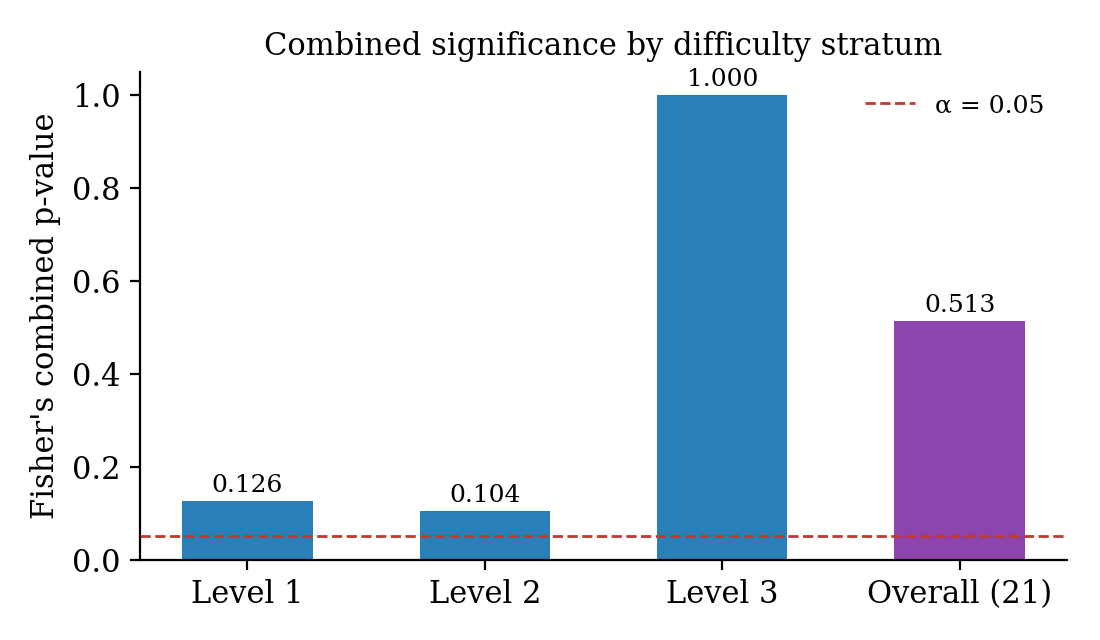
\includegraphics[width=0.6\textwidth]{figs/fig2_stratum_pvalues.png}
\caption{Fisher's combined $p$-value by difficulty stratum and overall. No stratum, nor the overall combined test, reaches the $\alpha=0.05$ threshold (dashed line).}
\label{fig:stratum}
\end{figure}

\subsection{Distribution of individual-pair results}
\label{sec:results-dist}

16 of 21 pairs (76\%) show \textbf{exactly} PDI $=0$. Both sides' 40 branches converged to the identical answer every time, regardless of which history produced the matched checkpoint. This is the modal outcome. For the large majority of matched checkpoints tested, the model's current answer is a sufficient statistic for its eventual answer.

The remaining 5 pairs show nonzero PDI, of which 3 reach nominal significance at $p<0.05$, shown in Table~\ref{tab:sig}.

\begin{table}[h]
\centering
\caption{Nominally significant pairs at L1 matching.}
\label{tab:sig}
\begin{tabular}{lcc}
\toprule
Problem & PDI & $p$ \\
\midrule
\texttt{d2\_prob1} & 0.373 & 0.0005 \\
\texttt{d1\_prob3} & 0.123 & 0.0025 \\
\texttt{d1\_prob1} & 0.061 & 0.021 \\
\bottomrule
\end{tabular}
\end{table}

With 21 independent tests at $\alpha=0.05$, roughly 1 false positive is expected under a true global null ($21 \times 0.05 \approx 1.05$), so 3 nominal hits is only marginally above this baseline. Applying a Bonferroni correction ($\alpha/21 \approx 0.0024$), only \texttt{d2\_prob1} survives.

\begin{figure}[h]
\centering
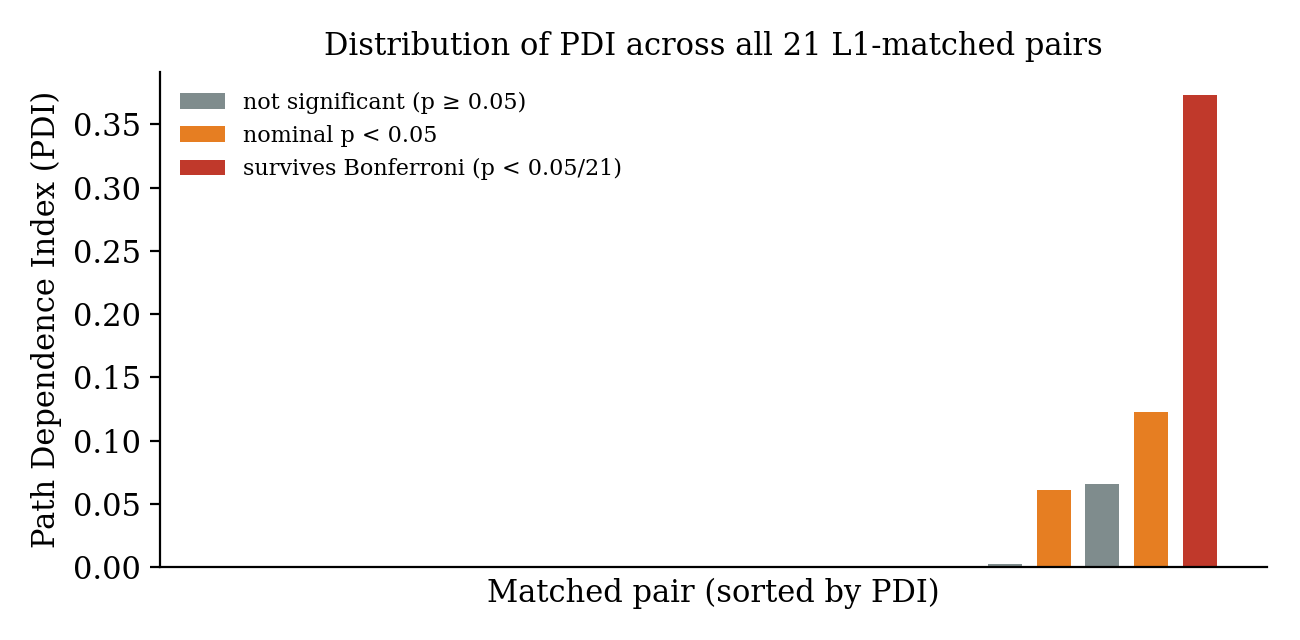
\includegraphics[width=0.6\textwidth]{figs/fig1_pdi_distribution.png}
\caption{PDI across all 21 matched pairs, sorted. 16 of 21 pairs show exactly PDI $=0$. Of the 5 nonzero pairs, only one (the tallest bar) survives Bonferroni correction across the 21 tests performed.}
\label{fig:pdidist}
\end{figure}

Two further pieces of evidence temper the remaining two pairs specifically.

\textbf{\texttt{d1\_prob3} is a measurement artifact, not a substantive divergence.} Inspecting the raw branch outputs, one side answered "2000" on 100\% of branches, while the other answered "2000" on 78\% and \textbf{"2000calories"} on 22\%, the same numeric answer with a units word included in the boxed content. This reflects a gap in our answer normalizer rather than a real divergence.

\textbf{\texttt{d1\_prob1} and \texttt{d2\_prob1} were each independently sampled twice} at the same matching level, as two distinct matched pairs per problem, drawn from different trajectory pairs. Neither replicated on its second draw. \texttt{d1\_prob1}'s other pair scored PDI $=0.0023$, $p=0.807$. \texttt{d2\_prob1}'s other pair scored PDI $=0.066$, $p=0.058$, just short of significance. Non-replication within the same problem and matching level, using data already collected rather than a new experiment, suggests these single-draw results should not be treated as a stable property of the problem.

\subsection{The two flagged pairs: raw pattern and why we read it as sparse-support noise}
\label{sec:results-flagged}

For the two nominally significant pairs that were not measurement artifacts (\texttt{d2\_prob1}, \texttt{d1\_prob1}), the raw branch outputs show neither reflects the model reaching a \emph{different} substantive answer depending on history. Both sides agree on which answer is correct. The split is in how often the model commits to stating it cleanly versus trailing off into an empty \texttt{\textbackslash boxed\{\}}, shown in Table~\ref{tab:decisive}.

\begin{table}[h]
\centering
\caption{Decisiveness gap for the two flagged anomalies at L1.}
\label{tab:decisive}
\begin{tabular}{lll}
\toprule
Problem & Side A & Side B \\
\midrule
\texttt{d2\_prob1} & 72.5\% "evelyn", 17.5\% empty, 10\% partial & 15\% "evelyn", \textbf{85\% empty} \\
\texttt{d1\_prob1} & 75\% "-50", 25\% empty & 95\% "-50", 5\% empty \\
\bottomrule
\end{tabular}
\end{table}

At face value this pattern, history predicting \emph{whether} an answer is stated rather than \emph{which} one, is an intuitive candidate mechanism, and we treated it as a live hypothesis through most of this project. We no longer read it as a real, stable phenomenon, for reasons that are all already in hand rather than speculative. First, neither pair survives Bonferroni correction once combined with the scale-up's 45 additional tests (Section~\ref{sec:results-scaleup}). Second, both source problems fail to replicate this pattern on an independently sampled second L1 pair at the same matching level (Section~\ref{sec:results-dist}). Third, the scale-up's 45 new pairs, drawn from a wider, harder pool of problems specifically to give this kind of effect more chances to recur, produced zero nominally significant pairs. Fourth, the continuous regression of divergence against state-space distance across all 66 pairs, the statistically appropriate test for exactly this question of whether richer state resolves the gap, is null (Section~\ref{sec:results-scaleup}). Taken together, this is what sparse-sample noise around a true null looks like when you get unlucky on 2 or 3 draws out of dozens, not what a real, mechanistically grounded effect looks like when you go looking for it again with more data and a better-powered test.

\subsection{A small discrete-matching check, superseded by the continuous test}
\label{sec:results-discrete-check}

Before running the scale-up, we performed a small, explicitly post-hoc check. We re-sampled matched pairs for these same two problems under L2 (plus confidence-matched) and L3 (plus entropy-matched) criteria, 1 pair per level per problem. Both pairs at both stricter levels came back with PDI $=0.000$.

\begin{figure}[h]
\centering
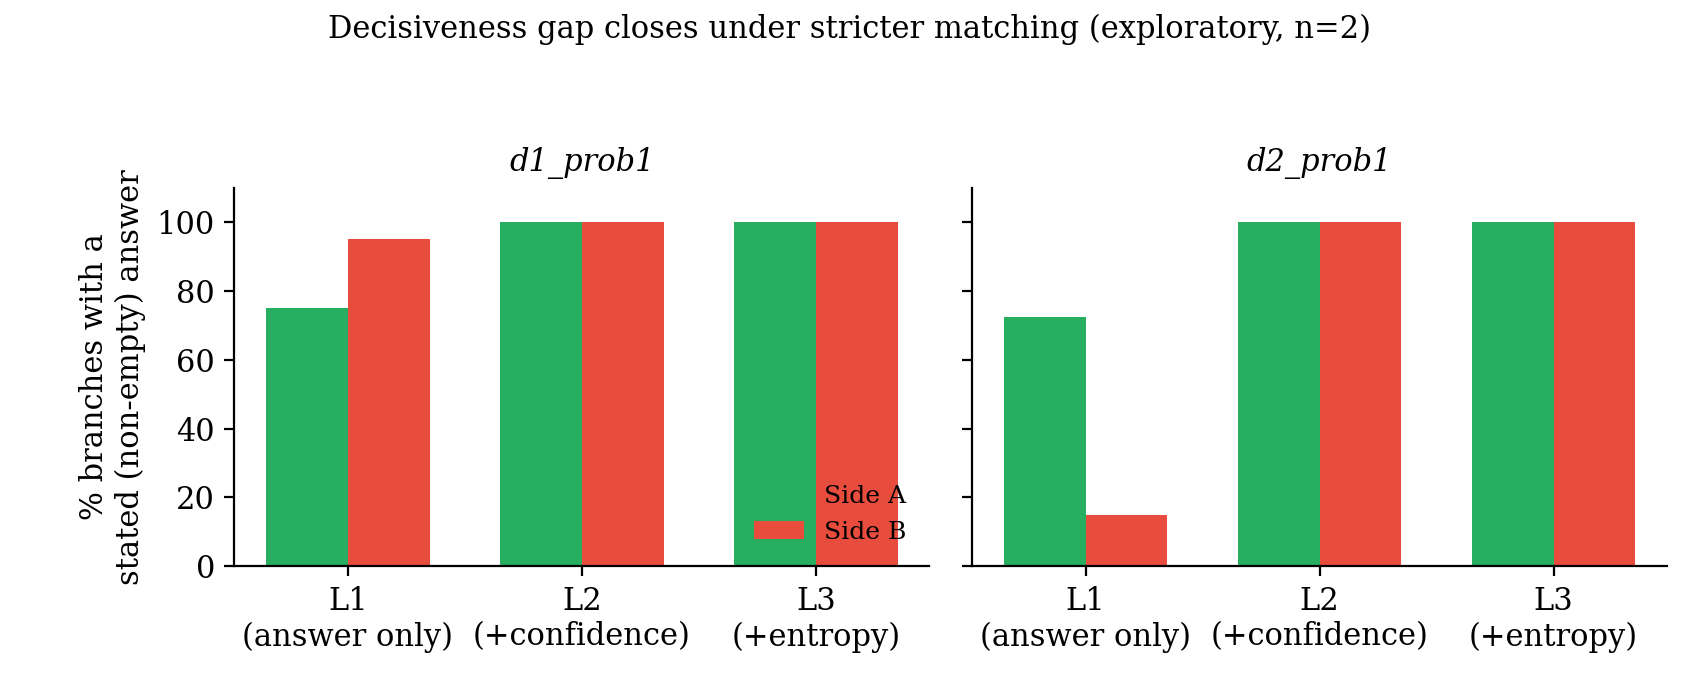
\includegraphics[width=0.85\textwidth]{figs/fig3_decisiveness_followup.png}
\caption{The two flagged anomalies' decisiveness gap (percentage of branches ending in a stated, non-empty answer) at L1, and the exploratory L2/L3 follow-up ($n=1$ pair per level per problem) where the gap closes.}
\label{fig:followup}
\end{figure}

At the time, we reported this only as suggestive ($n=2$ is not independently powered, and a null here is also what the problems' own noise floor predicts on its own). We include it here for completeness, but do not lean on it. Section~\ref{sec:results-scaleup}'s continuous regression is the statistically correct version of this same question, run at $n=66$ rather than $n=2$, and it is the result we treat as informative.

\subsection{Scale-up and the continuous state-distance regression}
\label{sec:results-scaleup}

To directly address whether the two flagged pairs in Section~\ref{sec:results-flagged} reflect a real effect, we collected an independent, additional 45 matched pairs (15 per MATH-500 difficulty level, levels 1 to 3), each branched under L1 matching and instrumented to save both sides' exact observable state and a hidden-state activation vector at the matched checkpoint, instrumentation the original pilot lacked (Section~\ref{sec:lim-scope}). Budget constraints for this round fixed the per-pair branch count at $N=10$ rather than the pre-registered $N=40$, so individual pairs in this scale-up are markedly lower-power than the primary sample. We treat it as a confirmatory check on aggregate patterns and as the dataset needed for the continuous regression below, not as a replacement for the primary 21-pair result.

\textbf{Scale-up result: zero nominally significant pairs.} 0 of 45 new pairs reach $p<0.05$ (Fisher-combined $p \approx 1.0$). 40 of 45 (89\%) show exactly PDI $=0$. Table~\ref{tab:scaleup} breaks this out by difficulty.

\begin{table}[h]
\centering
\caption{Scale-up results by MATH-500 difficulty level.}
\label{tab:scaleup}
\begin{tabular}{lccccc}
\toprule
Difficulty & $n$ pairs & Combined $p$ & Mean PDI & Exact-zero pairs \\
\midrule
Level 1 & 15 & 1.000 & 0.000 & 15/15 \\
Level 2 & 15 & 1.000 & 0.007 & 14/15 \\
Level 3 & 15 & 1.000 & 0.035 & 11/15 \\
\bottomrule
\end{tabular}
\end{table}

Difficulty level 3 shows more nonzero variance than levels 1 and 2, consistent with the a priori hypothesis in Section~\ref{sec:method-strat} that harder problems admit more divergent reasoning paths, but the combined test remains far from significant even restricted to this stratum. Pooling the original 21 pairs with these 45 ($n=66$ total, all L1-matched), the same three pairs from Section~\ref{sec:results-dist} remain the only nominal hits. No new significant pairs emerged from the scale-up, and the pooled Fisher-combined $p$ is 0.9999996. \texttt{d2\_prob1} survives Bonferroni correction at this pooled $n$ by a thin margin ($p=0.0005$ against a threshold of $0.05/66 \approx 0.00076$). Given the non-replication evidence in Sections~\ref{sec:results-dist} and \ref{sec:results-flagged}, we do not treat this survival as evidence of a real effect.

\textbf{The continuous regression, finally run.} An earlier draft of this paper identified, but had not run, a statistically stronger test than discrete L1/L2/L3 bucketing: regressing PDI directly against the continuous state-space distance between two matched prefixes, defined in Equation~\ref{eq:statedist}, pooling all matched pairs rather than comparing small discrete buckets. Fitting Equation~\ref{eq:regression} on the 45 pairs collected with state instrumentation (state distance was not recorded in the original 21-pair collection and cannot be reconstructed retroactively) gives
\begin{equation}
\hat\beta_1 = -0.0086, \quad r = -0.11, \quad p = 0.47 \quad (n = 45),
\end{equation}
with a 95\% confidence interval on the slope of $[-0.032, +0.015]$. Figure~\ref{fig:contreg} shows the fitted line and its 95\% confidence band against the raw scatter.

\begin{figure}[h]
\centering
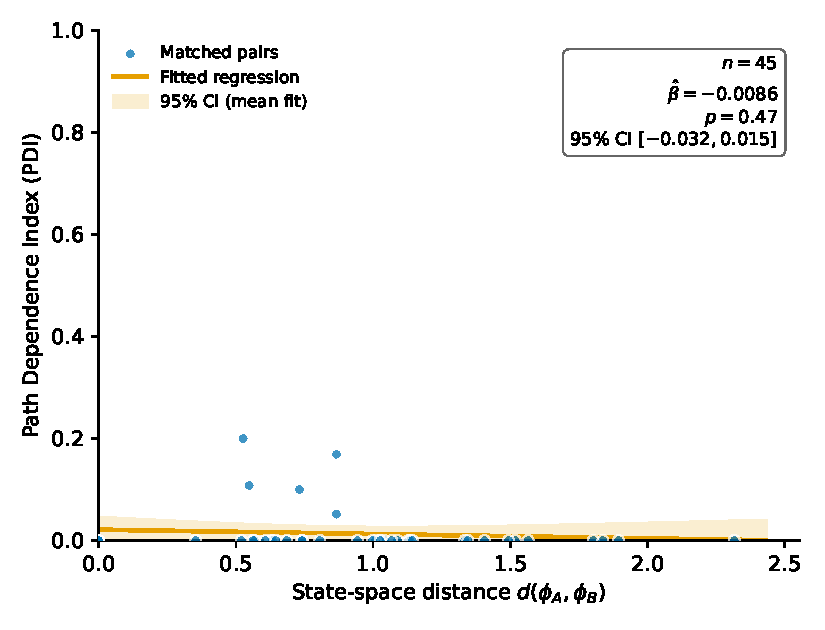
\includegraphics[width=0.62\textwidth]{figs/fig_continuous_regression.pdf}
\caption{Path Dependence Index against state-space distance for all 45 scale-up pairs, with the fitted regression line and its 95\% confidence band. The slope is flat and its 95\% confidence interval covers zero, showing no evidence of path dependence as a function of observable state distance.}
\label{fig:contreg}
\end{figure}

This is a null result, and if anything points the opposite direction from a path-dependence hypothesis. Pairs with \emph{more} distant states show slightly \emph{lower} divergence, not higher, though the effect is far too small and noisy to interpret as more than sampling variation around zero. We treat this as the strongest single piece of evidence in this paper for sufficiency. It is the test our own design flagged in advance as the correct one, run on real data, pooling far more information per test than the discrete comparisons in Section~\ref{sec:results-discrete-check}, and it agrees with every other test we ran.

\textbf{Mechanistic probe: uninformative, not negative.} We also attempted a hidden-state decisiveness probe motivated by Section~\ref{sec:results-flagged}'s original hypothesis, asking whether the property "will this prefix state a decisive answer" is linearly decodable from its hidden state. It could not be trained. Across all 90 labeled examples (45 pairs times 2 sides), every single branch set produced a non-empty answer. Zero "trails off empty" examples occurred at $N=10$ branches per pair, so the label has no variance for a classifier to learn from. We report this as a data-collection outcome, not a finding. The decisiveness failure mode this probe was built to study did not recur at this reduced branch budget, which is itself mildly consistent with Sections~\ref{sec:results-flagged} and~\ref{sec:results-scaleup}. Decisiveness gaps large enough to detect at $N=40$ branches may simply be rare, low-branch-count artifacts rather than a systematic property of any of these problems.

\subsection{Does a stopping rule built on these findings beat the simplest baseline?}
\label{sec:results-sges}

If current observable state is sufficient, the practical implication is that early-stopping methods do not need to track anything more sophisticated than simple answer and confidence extraction. Matching mechanisms more elaborate than that are solving a problem the data does not support having. We test this directly with \textbf{Sufficiency-Gated Early Stopping (SG-ES)}: stop generation the first time an answer has been stable for 2 consecutive scored steps \emph{and} confidence at that step exceeds 0.70, motivated directly by this paper's own L1 and L2 observations. We compare it against two baselines computed post-hoc from the same dense, step-scored trace, \textbf{full generation} (run to completion) and \textbf{forced extraction at a fixed 50\% depth} (the naive rule, ignoring confidence entirely), on 19 usable MATH-500 problems (levels 1 to 4, 5 of 24 sampled problems dropped for 0 scored prefixes, the same forced-extraction failure mode noted throughout this paper). Results are in Table~\ref{tab:sges}.

\begin{table}[h]
\centering
\caption{SG-ES compared with full generation and a naive fixed-fraction baseline.}
\label{tab:sges}
\begin{tabular}{lcc}
\toprule
Condition & Accuracy & Mean fraction of trace used \\
\midrule
Full generation & 0.842 & 1.000 \\
Forced extraction at 50\% (naive) & 0.842 & 0.687 \\
SG-ES (confidence and stability gated) & 0.842 & 0.813 \\
\bottomrule
\end{tabular}
\end{table}

All three conditions tie on accuracy. Critically, \textbf{SG-ES does not save more compute than the naive fixed-fraction baseline, it saves less} (81.3\% of the trace used versus 68.7\%), despite triggering on 18 of 19 problems. Figure~\ref{fig:sges} shows both metrics side by side, with standard error bars computed across the 19 problems.

\begin{figure}[h]
\centering
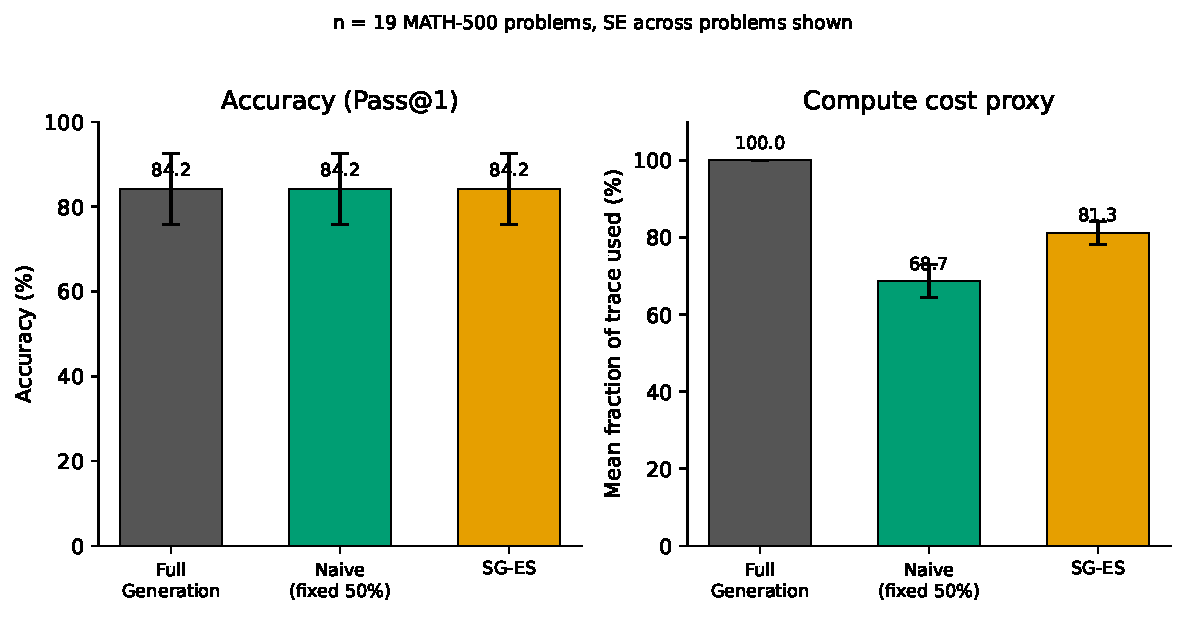
\includegraphics[width=0.85\textwidth]{figs/fig_sges_comparison.pdf}
\caption{Accuracy and compute cost (mean fraction of trace used, since raw token counts were not separately logged per condition) for full generation, the naive fixed-50\% baseline, and SG-ES, across 19 MATH-500 problems. Error bars show standard error across problems. SG-ES preserves full baseline accuracy but increases token consumption relative to naive early stopping.}
\label{fig:sges}
\end{figure}

This is the result we would predict if current answer state already carries what a stopping decision needs. Adding a confidence gate on top of simple answer-stability does not pay for itself here, and a substantially simpler rule matches it on both metrics that matter. We read this as corroborating, not merely consistent with, Section~\ref{sec:results-scaleup}'s central finding. It is what "state-matching sophistication beyond simple extraction is not buying anything" looks like in a live stopping-rule comparison, not only in a retrospective divergence test.

\section{Discussion: Why Might This Sufficiency Hold?}
\label{sec:discussion}

Everything in Section~\ref{sec:results} is a black-box behavioral result. We observe inputs and outputs, never gradients, attention, or routing internals (our one attempt to look inside, the hidden-state decisiveness probe in Section~\ref{sec:results-scaleup}, could not train on this round's data). What follows is therefore explicitly a \textbf{hypothesis for future mechanistic work, not a claim this paper tests}. We flag it as such throughout rather than letting the confident tone of the rest of the paper leak into speculation we have not verified.

\subsection{A training-time funneling hypothesis}
\label{sec:discussion-funnel}

DeepSeek-R1-Distill-Qwen-7B, the model used throughout this paper, is not itself RL-trained. As reported in the DeepSeek-R1 technical report \citep{deepseekr1_2025}, the distilled model family is produced by supervised fine-tuning of a Qwen2.5 base checkpoint on reasoning trajectories \emph{generated by} the RL-trained (GRPO) DeepSeek-R1 teacher. The 7B student never sees an RL objective directly. It imitates the teacher's already-produced outputs. This two-stage lineage suggests a candidate explanation for why our null holds, at least for this specific model.

GRPO optimizes the teacher's policy using a reward that is, in DeepSeek-R1's reported setup, a function of the \emph{final} answer's correctness (plus formatting), evaluated across a group of sampled rollouts from the same prompt and normalized within-group. Critically, this reward signal has no mechanism to distinguish between two rollouts that reach the same correct answer by different reasoning paths. RL gradient pressure under this objective can shape \emph{when and how confidently} a trajectory commits to an answer, but has no way to independently reward or penalize \emph{which path} it took to get there, once the destination is fixed. If this group-relative, outcome-only objective causes the teacher's policy to converge many different reasoning paths onto a narrow, low-variance continuation distribution once enough evidence has accumulated for a given answer, a plausible mechanism, though not one we test directly, then the teacher's own training data, used to fine-tune the distilled student, would already exhibit exactly the behavioral pattern this paper measures: path-independence of future output conditional on current $\phi(p)$. The student, trained only to imitate that already-funneled distribution, would inherit the pattern without needing any RL stage of its own.

This framing makes a falsifiable prediction for future work, which we regard as the most direct way to test the hypothesis rather than just argue for it. \textbf{Path dependence, if it exists, should be more likely to appear in models whose training does not include this kind of outcome-only, group-relative shaping}, for example a base model continuing raw chain-of-thought with no reasoning-specific fine-tuning, or a policy trained with an explicit diversity or entropy bonus over intermediate reasoning rather than an outcome-only reward. Our finding would then be best read not as a property of "reasoning models" as a category, but as a downstream consequence of a specific, now-common training recipe, a sharper and more useful claim than the more general one, and consistent with the generalization caution in Section~\ref{sec:lim-general}.

\subsection{Reconciling with RAD: representational divergence without behavioral divergence}
\label{sec:discussion-rad}

RAD \citep{rad2026} (Section~\ref{sec:relatedwork}) reports that identical output tokens do not imply identical internal state. Hidden activations and mixture-of-experts routing decisions can differ even when the surface token stream matches. Taken at face value, this could look like it contradicts our finding. If internal state still diverges after two trajectories agree on a token, how can we also find that their \emph{future} behavior converges regardless of history?

We think these findings are compatible, not in tension, once "state" is disambiguated. Our $\phi(p)$ is a deliberately low-dimensional, behaviorally defined summary (answer, confidence, entropy), a projection of whatever the model's full internal state is, chosen because it is exactly what existing early-stopping methods already compute and act on. RAD's internal state is much higher-dimensional and representationally complete. It is entirely possible, and if RAD's finding holds, likely, for the full internal state to remain genuinely path-dependent, meaning the model "remembers," in its activations or routing, something about how it got here, while that residual memory is behaviorally inert for the specific downstream question this paper asks: what final answer will this trajectory eventually state. A sufficient statistic is only sufficient \emph{for a specific target}. $\phi(p)$ can be sufficient for predicting the eventual answer while being insufficient for predicting other properties (response style, verbosity, robustness to a rephrased question, or exactly the routing-level facts RAD's probing methodology is built to detect) that a hidden-state-level analysis would still find path-dependent.

This is also, concretely, what our own attempted hidden-state decisiveness probe (Section~\ref{sec:results-scaleup}) was designed to test, whether hidden state carries decisiveness-relevant information \emph{beyond} $\phi(p)$, and it remains the most direct way to adjudicate this question on our own data and pipeline, rather than by analogy to a different paper's setup. It could not train this round because the label had no variance at $N=10$ branches. Rerunning it at the pre-registered $N=40$, specifically targeting problems and matching levels known to produce some non-decisive branches (\texttt{d2\_prob1} and \texttt{d1\_prob1} from Section~\ref{sec:results-dist}), is the concrete next experiment we would run to test this section's hypothesis directly rather than only discuss it.

\section{Limitations and Future Work}
\label{sec:limitations}

\subsection{Scope: discrete matching levels remain L1-only}
\label{sec:lim-scope}

Our design pre-registered testing discrete L1, L2, and L3 matching and reporting whether richer state resolves any gap found at the loosest level. Due to an implementation bug, the pair-branching loop shared one sampling budget across all three matching levels instead of giving each an independent budget, so L1 always exhausted it before L2 or L3 were ever sampled. \textbf{All 66 pairs in this paper (21 primary plus 45 scale-up) are L1 (answer-only) matched.} The bug itself is fixed and verified, since the follow-up L2/L3 collection in Section~\ref{sec:results-discrete-check} used the corrected code path successfully, but we did not spend further budget on a full L2/L3 stratified sweep at scale, because Section~\ref{sec:results-scaleup}'s continuous state-distance regression answers the underlying question directly and more informatively than discrete L2/L3 buckets would, without needing separate matching-level datasets. \textbf{The one thing that remains genuinely untested is whether a full-scale discrete L2/L3 design would qualitatively agree with the continuous regression.} We have no reason to expect it would disagree, but we have not run it and do not claim otherwise.

\subsection{Achieved sample size: 21 of 24 pre-registered pairs}
\label{sec:lim-samplesize}

One difficulty-3 chunk's two problems initially produced 0 usable matched pairs (0 of 500 forced-extractions parsed), because the natural reasoning trace was truncating before reaching a conclusion at the original 2000-token budget, triggering our own pre-registered inconclusive-data flag. We diagnosed and fixed this by raising the trace and scoring token budgets and reran, but the rerun yielded only 1 pair for that chunk rather than the targeted 3, leaving the final dataset 3 pairs short of the 24-pair target. We report the achieved sample of 21 pairs (7 per stratum) rather than treating 24 as met.

\subsection{Statistical caution on the flagged pairs}
\label{sec:lim-caution}

As detailed in Sections~\ref{sec:results-dist} and~\ref{sec:results-flagged}, of the 3 nominally significant pairs in the primary sample, only \texttt{d2\_prob1} survives Bonferroni correction, and only by a thin margin once the correction is computed across the pooled 66-pair set rather than the original 21. Combined with both flagged problems' failure to replicate on a second independently sampled pair, the scale-up's zero new significant pairs out of 45, and the continuous regression's null result, we now read this as resolved. The original flags are consistent with sparse-sample noise, not a stable effect we failed to fully characterize. We still regard the broader lesson as generalizable. Any future work using this kind of design should budget for within-condition replicates and, ideally, the continuous-distance regression from the start, rather than treating a single significant discrete-bucket pair as a finding.

\subsection{The continuous test has now been run}
\label{sec:lim-continuous}

Section~\ref{sec:results-scaleup} reports the continuous state-distance regression this section previously flagged as identified but not run. It required persisting per-pair observable state and hidden-state vectors, which the original 21-pair collection did not do and which we added via new instrumentation for the 45-pair scale-up. The regression is null ($p=0.47$, $n=45$) and agrees with every other test in this paper. What remains open is that this regression pools only the 45 scale-up pairs, since the 21 primary pairs lack saved state and cannot be added retroactively, it was run at a reduced $N=10$ branches per pair rather than the pre-registered 40, and, like everything else in this paper, it reflects one model on one domain. A higher-power replication of the continuous regression specifically, with state persisted from the start and the full $N=40$ branch budget, is the most direct way to raise confidence in this paper's central claim beyond what we report here.

\subsection{Generalization}
\label{sec:lim-general}

All results, the primary sample, the scale-up, the continuous regression, and the SG-ES comparison, are from a single model (DeepSeek-R1-Distill-Qwen-7B) on a single dataset (MATH-500). We report a well-powered null within this scope. We do not claim it as a general proof that observable state is sufficient across reasoning model families, sizes, or task domains (for example GSM8K or commonsense reasoning), and readers should not extend our framing that far on their own. A null result of this kind licenses the claim that current-state early-stopping is not obviously leaving exploitable history on the table, for this model and this domain, not the claim that history never matters, anywhere.

\subsection{Pipeline reliability}
\label{sec:lim-pipeline}

Over the course of this pilot we found and fixed several implementation bugs that materially affected results before being caught, including a library version incompatibility that silently crashed generation, an auto-selected numerical precision that degraded output quality by 65 to 82\% before being pinned explicitly, and the matching-level budget bug in Section~\ref{sec:lim-scope}. We do not consider the current pipeline guaranteed free of further such issues, and note this as a general caution for interpreting any single pilot's numbers as final, particularly ones, like this one, run under a fixed compute budget across heterogeneous infrastructure.

\subsection{Anticipated objections}
\label{sec:lim-objections}

We list the three critiques of this design we consider most serious, in our own words as if made by a skeptical reviewer, and respond to each directly rather than only in aggregate.

\textbf{Objection 1.} The 45-pair scale-up was run at $N=10$ branches per pair, a quarter of the pre-registered $N=40$ that Section~\ref{sec:method-power}'s own power analysis said was necessary. At $N=15$, that analysis measured only 3 to 9\% power to detect the targeted effect size, regardless of pair count. A scale-up that cannot detect a true effect of the size this paper cares about cannot meaningfully confirm a null. 0 of 45 significant pairs is close to the guaranteed outcome of an underpowered design, not evidence for anything.

This is correct as stated about \emph{per-pair} significance testing, and we do not dispute the power math. We do not claim any individual pair in the scale-up is independently powered to detect the pre-registered effect size, and say so explicitly in Sections~\ref{sec:method-scaleup} and~\ref{sec:results-scaleup}. But per-pair significance is not the test we are asking the scale-up to carry. Its two actual jobs are, first, supplying pooled data to the continuous state-distance regression, whose power comes from the number and spread of distance and PDI observations rather than any single pair's branch count, and second, an aggregate check (fraction exactly-zero, combined Fisher $p$) that is informative about the \emph{distribution} of outcomes even when no single pair in it is a confirmatory test on its own. On the regression specifically, we can report realized precision directly rather than ask the reader to infer it from a per-pair calculation designed for a different test. The 95\% confidence interval on the fitted slope is $[-0.032, +0.015]$ (change in observed PDI per unit state distance), and the observed state-distance range in this data is 0 to 2.32. Projected across that full observed range, this interval rules out, at 95\% confidence, a monotonic PDI effect larger than roughly $-0.075$ to $+0.035$, a substantial fraction of the 0 to about 0.20 PDI range we actually observed in this data. That is a real, checkable precision statement, not an appeal to the scale-up's aggregate size. We agree this is not as strong as a properly powered replication at $N=40$ would be, and say exactly that in Section~\ref{sec:lim-continuous}. The single most valuable follow-up to this paper is that replication, not a defense of the current one.

\textbf{Objection 2.} The paper is framed around observable state sufficiency in general, but the only well-powered test, the primary 21-pair sample, uses L1 (answer-only) matching exclusively, due to the budget bug in Section~\ref{sec:lim-scope}. A reader could reasonably think confidence and entropy were tested with the same rigor as the answer, when in fact the only test that touches them directly is the lower-power, $N=10$ continuous regression.

This is a fair and precise criticism, and we have tried to make the paper's own language track it rather than paper over it. Section~\ref{sec:results-primary}'s headline result is stated as a null under answer-only matching, not as a general sufficiency claim, and the abstract and introduction both explicitly scope the well-powered claim to L1 while separately and honestly flagging the continuous regression's reduced power. We do not believe the paper currently overstates what the confidence and entropy axis specifically has been shown, and we would consider it a legitimate revision request to make this distinction even more prominent. The concrete fix, not yet run, is a full-scale discrete L2/L3 sweep or a continuous regression at the pre-registered $N=40$, both already listed as the paper's top future-work item.

\textbf{Objection 3.} DeepSeek-R1-Distill-Qwen-7B is a distilled model, trained via supervised fine-tuning on a teacher's already-generated reasoning traces. Output homogeneity, meaning low diversity and a narrow trajectory distribution, is a known property of distillation generally. A near-zero path-dependence result on a model whose training objective may already collapse trajectory diversity could simply be measuring the distillation process, not a general property of reasoning models, and would not be expected to replicate on a directly RL-trained, non-distilled model with a more diverse rollout distribution.

This is, in our own assessment, the single largest external-validity threat to this paper, and Section~\ref{sec:discussion-funnel}'s discussion engages it head-on rather than treating it as a footnote. We propose training lineage, meaning outcome-only, group-relative RL shaping the teacher, then supervised fine-tuning distilling that into the student, as a \emph{candidate mechanism} for our null, which, if correct, predicts our finding is a property of this training recipe, not of reasoning models generally. We did not test a non-distilled, directly RL-trained model in this paper, and we do not claim our result generalizes to one. We regard replicating this design on a model such as the full DeepSeek-R1 or another directly RL-trained reasoning model, specifically to test whether path dependence reappears outside the distillation setting, as the most theoretically interesting single follow-up this paper motivates, more interesting, in fact, than replicating on the same class of model at higher power, because it tests the \emph{mechanism} in Section~\ref{sec:discussion-funnel} rather than just this paper's statistical confidence in its own model-specific result.

\section*{Reproducibility Statement}

All experiments use a single open-source model, \textbf{DeepSeek-R1-Distill-Qwen-7B} (publicly available checkpoint, no fine-tuning applied), and a single public benchmark, \textbf{MATH-500}. Trajectory generation uses temperature 0.6 throughout, at fp16 precision, forced explicitly rather than auto-selected. An earlier auto-selected bf16 run on different hardware degraded output quality by 65 to 82\% before this was caught and pinned (Section~\ref{sec:lim-pipeline}). Top-$p$ is explicitly set to 0.95 in the generation config used for the pre-registered 21-pair primary sample. The 45-pair scale-up and the SG-ES evaluation use the same temperature but do not explicitly override top-$p$, relying instead on the checkpoint's own default generation config. We did not verify this resolves to the same value and flag it here as a genuine configuration difference between the two collection tracks rather than assume equivalence. A fully precise replication of the primary sample should pin \texttt{top\_p=0.95} explicitly, as the released generation scripts for that track do.

Token budgets are up to 3000 new tokens for full reasoning trajectories (2000 for the majority collected before a one-difficulty-stratum-specific increase, documented in Section~\ref{sec:lim-samplesize}), up to 64 new tokens for forced-extraction $\phi(p)$ scoring, and up to 1500 new tokens per natural branch continuation. Matching tolerances are confidence at most 0.10 for L2, entropy at most 0.15 for L3, and normalized depth at most 0.15 at all levels. Branch counts are $N=40$ per side for the pre-registered 21-pair primary sample and the exploratory L2/L3 follow-up, and $N=10$ per side for the 45-pair scale-up and the SG-ES evaluation, a reduced budget whose effect on statistical power is discussed explicitly in Section~\ref{sec:lim-objections}. The permutation null for the Path Dependence Index uses 2000 resplits per pair. Difficulty stratification uses MATH-500's own provided level field (values 1 through 4).

All trajectory-generation and branching scripts, the forced-extraction $\phi(p)$ scoring code, the continuous state-distance regression code, the SG-ES stopping-rule implementation and its unit tests, the hidden-state-decisiveness logistic-regression probe, and the raw parsed branch-outcome logs underlying every number and figure in this paper are released at \url{https://github.com/Sharkyii/cot-path-dependence}.

\bibliographystyle{plainnat}
\bibliography{references}

\end{document}
